\documentclass[12pt,a4paper,oneside]{article}
\usepackage{amsmath,amsthm,amsfonts,amssymb}
\usepackage{pst-eucl,pstricks,pstricks-add}
\usepackage[utf8]{inputenc}
%\usepackage[latin1]{inputenc}
\usepackage[spanish,activeacute]{babel}
\usepackage[a4paper,margin=2.5cm]{geometry}
\usepackage{times}
\usepackage[T1]{fontenc}
\usepackage{titlesec}
\usepackage{color}
\usepackage{url}
\usepackage{float}
\usepackage{cite}
\usepackage{graphicx}
\usepackage{multicol}
\usepackage{lipsum}
\usepackage{transparent}
\usepackage{eso-pic}
%\AddToShipoutPicture*{
   % \put(0,0){
        %\parbox[b][\paperheight]{\paperwidth}{%
           % \vfill
            %\centering
            %{\transparent{0.5}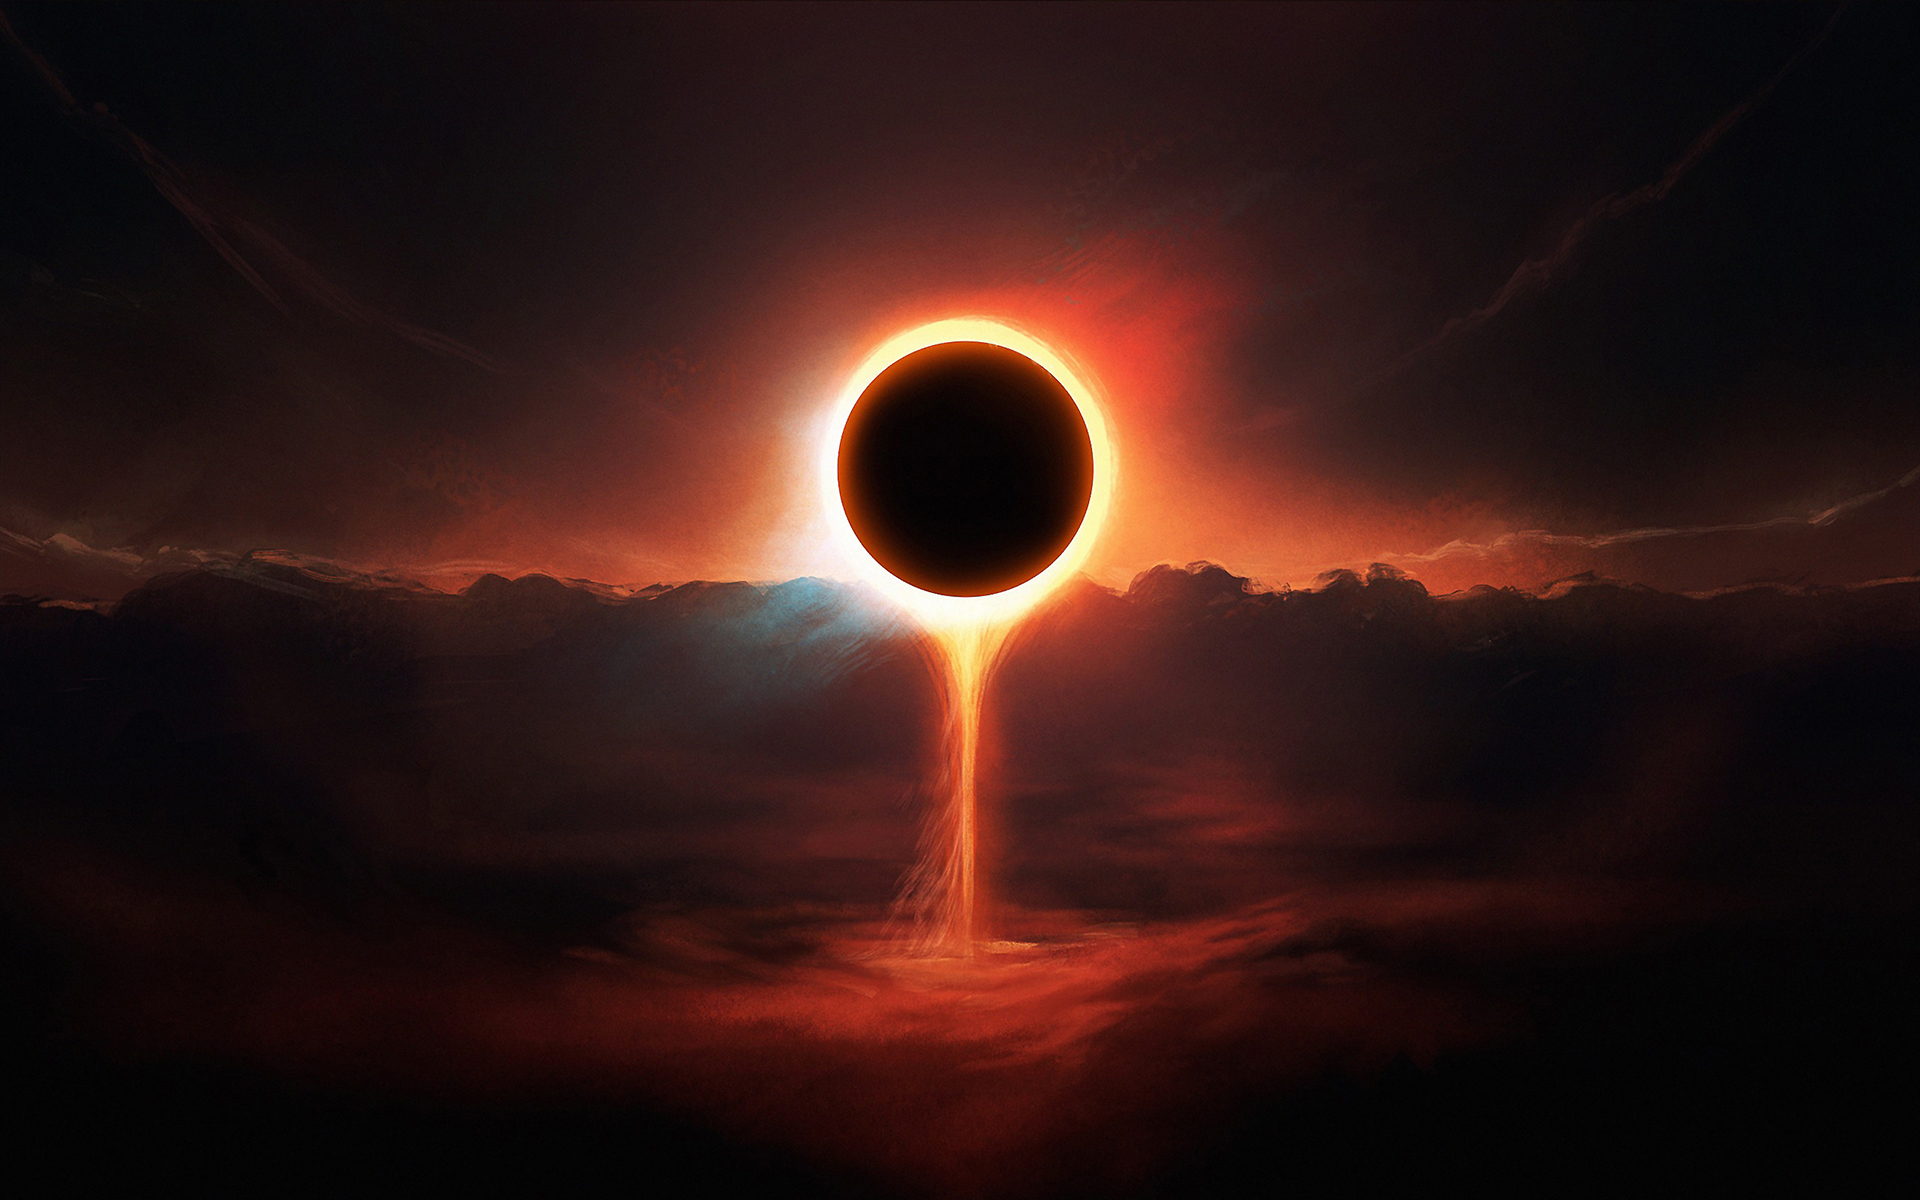
\includegraphics[width=3.5\textwidth]{febrero}}%
           % \vfill
       % }
   % }
%}
%\AddToShipoutPicture*{
   % \put(0,0){
      %  \parbox[b][\paperheight]{\paperwidth}{%
           % \vfill
           % \centering
           % {\transparent{0.5}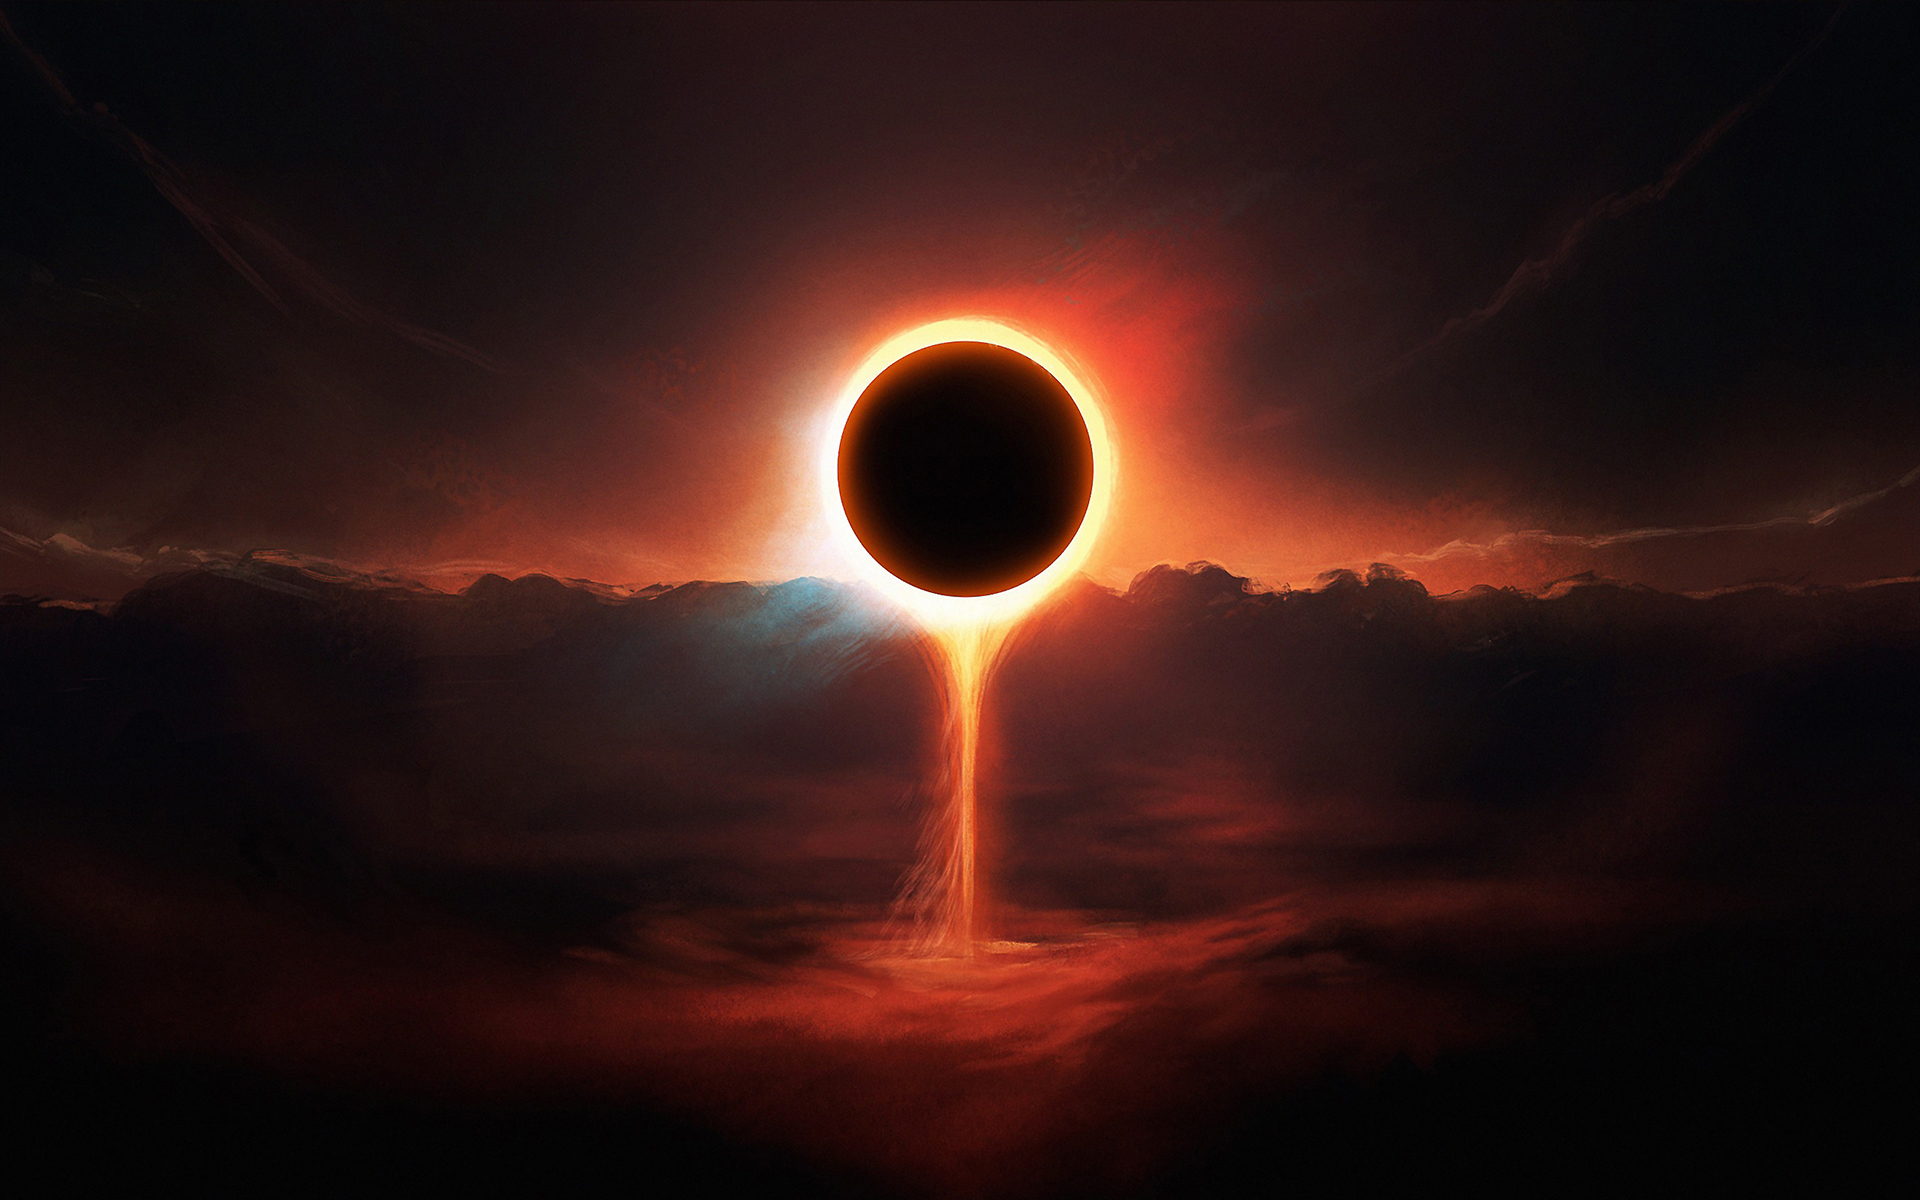
\includegraphics[width=3\textwidth]{febrero}}%
          %  \vfill
       % }
    %}
%}

\usepackage{draftwatermark}
\SetWatermarkText{\transparent{0.4}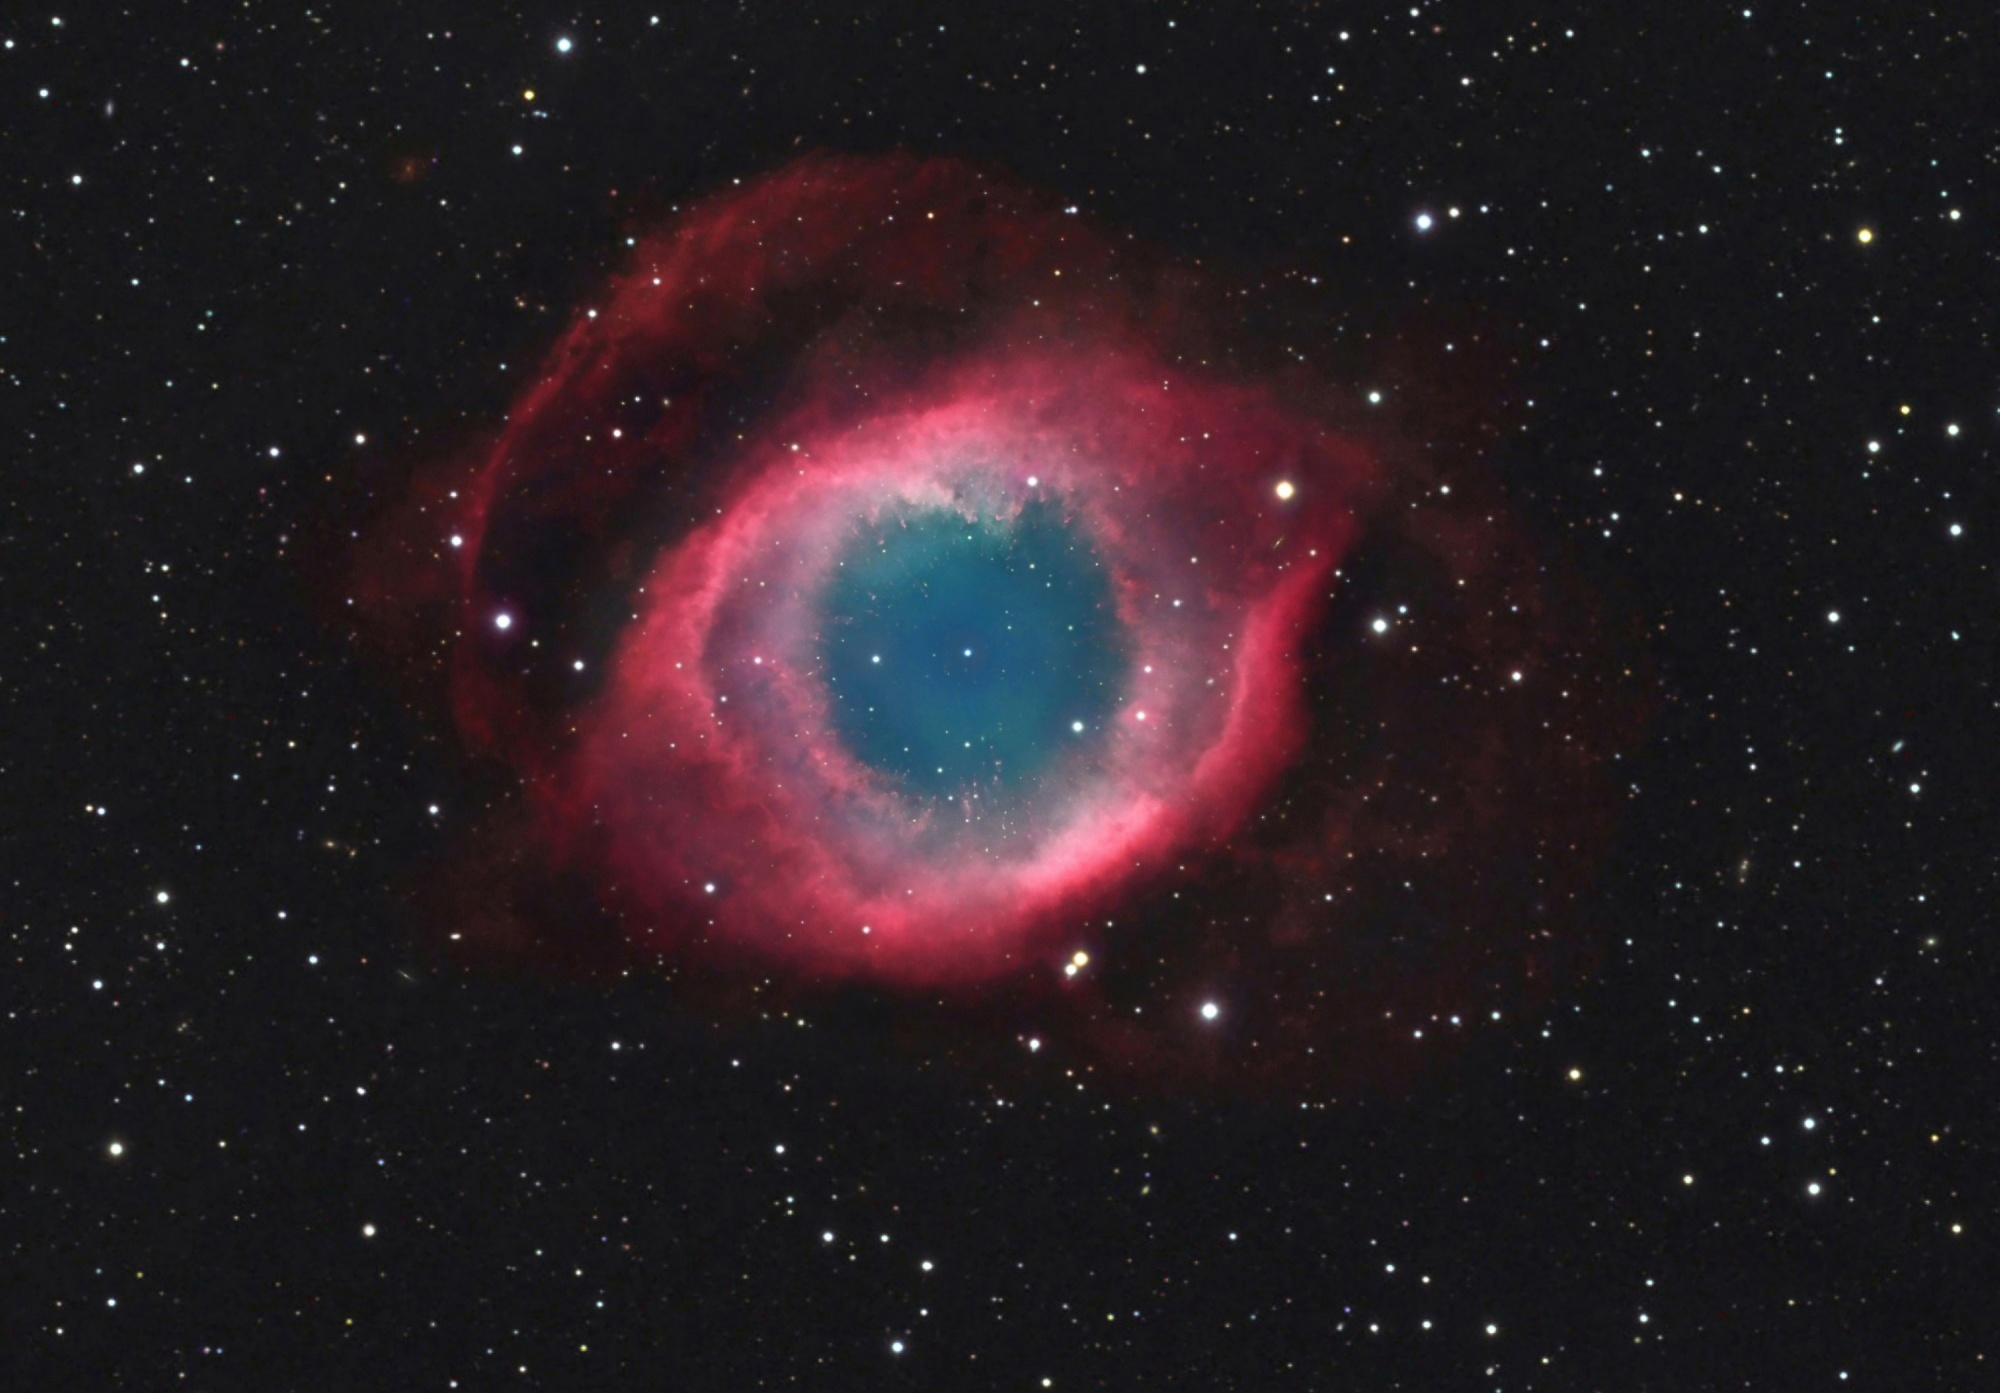
\includegraphics[scale=0.9,trim={5cm 0 5cm 0},clip,angle=-45]{helix}}
\usepackage{gensymb}
\usepackage{hyperref}
\usepackage{setspace}%\doublespace %para doble espacio
\onehalfspace %para espacio y medio
\newcommand{\code}[1]{\fcolorbox{blue!80}{gray!10}{#1}}
\parindent=0mm
\begin{document}
%\SweaveOpts{concordance=TRUE}
\rule[1mm]{170mm}{0.20mm}
\begin{minipage}[d]{30mm}
\begin{center}

\includegraphics[scale=0.30]{logo_epn.png}
\end{center}
\end{minipage}
\begin{minipage}[d]{100mm}
\begin{center}
\vspace{0.5cm}
\textsf{\textbf{\large ESCUELA POLITÉCNICA NACIONAL}}\\
\textsf{\textbf{\small OBSERVATORIO ASTRONÓMICO DE QUITO}}\\
\end{center}
\end{minipage}
\begin{minipage}[d]{30mm}
\begin{center}
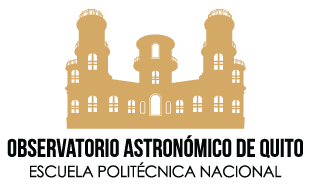
\includegraphics[scale=.40]{logo.png}
\end{center}
\end{minipage}\\
\rule[1mm]{170mm}{0.20mm}
\begin{center}
\textbf{\huge EFEM\'ERIDES ASTRON\'OMICAS 2017 \\}
\vspace{1cm}
\end{center}
\section{ENERO}
\begin{center}
\begin{tabular}{ |l| l| l| }
\hline
 \textbf{Fecha} & \textbf{Hora} & \textbf{Evento}\\
 \hline
 01/01/2017& 01:39:16 &	Marte a $0.02 \degree S$ de Neptuno. (Elongación mínima de los planetas: $58.7 \degree $)	\\
01/01/2017&01:52:38 &	Marte a $0.02 \degree $ de Neptuno. (Elongación mínima de los planetas: $58.7 \degree $)	\\
02/01/2017&22:59:52 &	Ocultación de Neptuno por la Luna. DM: 0.396 Ilum: $22.8\%$ \\
03/01/2017&01:38:17 &	Ocultación de Marte por la Luna. DM: 0.245 Ilum: $23.7\%$\\
04/01/2017& 09:17:50 &	Tierra en el perihelio. (Distancia heliocéntrica: 0.98331 U.A.)	\\
05/01/2017&14:47:00 &	Cuarto creciente (Distancia geocéntrica:373554 Km.)	\\
05/01/2017&22:44:10 &	Urano a $2.94 \degree N$ de la Luna. (Altura solar: $-57.3 \degree $)\\
06/01/2017&00:21:43 &	Urano a $2.79 \degree $ de la Luna. (Altura solar: $-67.2 \degree $)\\
08/01/2017&04:36:39 &	Mercurio estacionario. (Elongación: $19.7 \degree $)\\
10/01/2017&01:00:51 &	Luna en el perigeo. (Distancia geocéntrica: 363238 Km | Iluminación: $92.9\%)$\\
12/01/2017&06:33:58 &	Luna llena (Distancia geocéntrica:366879 Km.)	\\
12/01/2017&16:53:48 &	Venus a $0.36 \degree $ de Neptuno. (Elongación mínima de los planetas: $47.1 \degree $)	\\
12/01/2017&20:45:04 &	Venus a $0.41 \degree N$ de Neptuno. (Elongación mínima de los planetas: $47.0 \degree $)	\\
17/01/2017&03:35:08 &	Máxima extensión iluminada de Mercurio. (Fase: $79.75 \degree $Elo: $24.02 \degree $ O V=-0.1)	\\
19/01/2017& 01:01:08 &	Júpiter a $2.82 \degree $ de la Luna. (Altura solar: $-67.5 \degree $)\\
19/01/2017& 04:31:33 &	Mercurio en máxima elongación oeste. (Elongación: $24.13 \degree $)	\\
19/01/2017& 17:13:28 &	Cuarto menguante (Distancia geocéntrica:402139 Km.)	\\
21/01/2017&19:13:43 &	Luna en el apogeo. (Distancia geocéntrica: 404914 Km | Iluminación: $31.0\%$)	\\
24/01/2017&05:38:41 &	Saturno a $3.58 \degree $ de la Luna. (Altura solar: $-10.6 \degree $)	\\
27/01/2017&19:07:01 &	Luna nueva (Distancia geocéntrica:389614 Km.)	\\
30/01/2017&06:19:04 &	Ocultación de Neptuno por la Luna. DM: 0.198 Ilum: $6.7\%$ \\
\hline
\end{tabular}
\end{center}
\vspace{1cm}
\textbf{NOTA:  }\textit{Todos los eventos son calculados para la ubicaci\'on de la ciudad de Quito, y las horas se encuentran en hora local(LT=UTC-5)}
\vspace{0.7cm}
\newpage
\section{FEBRERO}
\begin{center}
\begin{tabular}{ |l| l| l| }
\hline
 \textbf{Fecha} & \textbf{Hora} & \textbf{Evento}\\
 \hline
 03/02/2017&23:18:53 &Cuarto creciente (Distancia geocéntrica:370623 Km.)	\\
06/02/2017&00:43:50 &	Júpiter estacionario. (Elongación: $114.5 \degree $)	\\
06/02/2017& 09:02:14&	Luna en el perigeo. (Distancia geocéntrica: 368816 Km | Iluminación: $76.4\%$)\\
07/02/2017&09:15:22&Mercurio en el afelio. (Distancia heliocéntrica: 0.46670 U.A.)	\\
10/02/2017&19:32:53 &	Luna llena (Distancia geocéntrica:377420 Km.)	\\
\colorbox{blue}{10/02/2017&19:44:03 &	Eclipse penumbral de Luna Visibilidad:Sin principio Magnitud:-0.03}\\
17/02/2017&01:43:31 &	Máxima extensión iluminada de Venus. (Fase: $116.94 \degree $ Diam: 39.08" \\
17/02/2017&02:17:11 &	Júpiter en el afelio. (Distancia heliocéntrica: 5.45652 U.A.)\\
18/02/2017&14:33:08 &	Cuarto menguante (Distancia geocéntrica:404373 Km.)\\
18/02/2017& 16:13:45 &	Luna en el apogeo. (Distancia geocéntrica: 404376 Km | Iluminación: $49.5\%$)	\\
20/02/2017&11:54:56 &	Venus en el perihelio. (Distancia heliocéntrica: 0.71845 U.A.)	\\
26/02/2017&09:53:25 &	Eclipse de sol   (Anular: No visible) \\
26/02/2017&09:58:22 &	Luna nueva (Distancia geocéntrica:378196 Km.)	\\
26/02/2017&15:56:29 &	Ocultación de Neptuno por la Luna. DM: 0.098 Ilum: $0.1\%$ \\
26/02/2017&17:26:16 &	Neptuno a $0.33 \degree $ de la Luna. (Altura solar: $15.0 \degree $)	\\
26/02/2017&17:43:01 &	Neptuno a $0.36 \degree $S de la Luna. (Altura solar: $10.9 \degree $)	\\
26/02/2017&19:19:18 &	Marte a $0.57 \degree $ de Urano. (Elongación mínima de los planetas: $43.4 \degree $)	\\
27/02/2017&03:23:10 &	Marte a $0.62 \degree N$ de Urano. (Elongación mínima de los planetas: $43.1 \degree $)\\
28/02/2017&15:34:50 &	Venus a $10.13 \degree N$ de la Luna. (Altura solar: $42.5 \degree $)	\\
\hline
\end{tabular}
\end{center}
\vspace{1cm}
\textbf{NOTA:  }\textit{Todos los eventos son calculados para la ubicaci\'on de la ciudad de Quito, y las horas se encuentran en hora local(LT=UTC-5)}
\vspace{0.7cm}
\newpage
\section{MARZO}
\begin{center}
\begin{tabular}{ |l| l| l| }
\hline
 \textbf{Fecha} & \textbf{Hora} & \textbf{Evento}\\
 \hline
01/03/2017& 09:27:07 &	Urano a $3.89\degree N$ de la Luna. (Altura solar: $44.8\degree$)	\\
01/03/2017& 13:01:46 &	Marte a $4.42\degree N$ de la Luna. (Altura solar:$ 78.7\degree$)	\\
01/03/2017& 21:45:30 &	Neptuno en conjunción. (Distancia geocéntrica:30.94145 U.A.)	\\
03/03/2017& 02:33:03 &	Luna en el perigeo. (Distancia geocéntrica: 369062 Km | Iluminación:$ 26.2\%$)	\\
04/03/2017& 00:30:12 &	Mercurio a $1.13\degree S$ de Neptuno. (Elongación mínima: $2.2\degree$)	\\
04/03/2017& 04:05:00 &	Venus estacionario. (Elongación: $29.9\degree$)	\\
04/03/2017& 06:10:03 &	Mercurio a 1.03\degree de Neptuno. (Elongación mínima de los planetas: $2.4\degree$)	\\
05/03/2017& 06:32:22 &	Cuarto creciente (Distancia geocéntrica:370468 Km.)	\\
06/03/2017& 19:14:07 &	Mercurio en conjunción superior. (Distancia geocéntrica: 1.36317 U.A.)	\\
12/03/2017& 09:53:48 &	Luna llena (Distancia geocéntrica:388858 Km.)	\\
16/03/2017& 18:17:11 &	Mercurio a $9.55\degree S$ de Venus. (Elongación mínima de los planetas: $9.5\degree$)	\\
18/03/2017& 07:27:01 &	Mercurio a $8.54\degree$ de Venus. (Elongación mínima: $11.0\degree$)	\\
18/03/2017& 12:25:27 &	Luna en el apogeo. (Distancia geocéntrica: 404650 Km | Iluminación: $68.1\%$)	\\
20/03/2017& 04:53:01 &	Saturno a $3.18\degree S$ de la Luna. (Altura solar: $-21.7\degree$)	\\
20/03/2017& 05:28:41 &	Inicio primavera	\\
20/03/2017& 06:10:24 &	Saturno a $3.15\degree$ de la Luna. (Altura solar: $-2.2\degree$)	\\
20/03/2017& 10:58:13 &	Cuarto menguante (Distancia geocéntrica:402269 Km.)	\\
22/03/2017& 11:39:24 &	Máxima extensión iluminada de Mercurio. Fase: $55.06\degree$ Diam: 5.90''	\\
23/03/2017& 08:53:17 &	Mercurio en el perihelio. (Distancia heliocéntrica: 0.30750 U.A.)	\\
25/03/2017& 05:11:25 &	Venus en conjunción inferior. (Distancia geocéntrica: 0.28107 U.A.)	\\
26/03/2017& 03:22:58 &	Ocultación de Neptuno por la Luna. DM: 0.005 Ilum: $4.1\%$ \\
26/03/2017& 10:05:44 &	Mercurio a $2.12\degree$ de Urano. (Elongación mínima: $17.3\degree$)	\\
27/03/2017& 00:56:17 &	Mercurio a $2.41\degree N$ de Urano. (Elongación mínima: $16.7\degree  $)	\\
27/03/2017& 06:00:32 &	Venus a $11.66\degree N $de la Luna. (Altura solar: $-4.2\degree$)	\\
27/03/2017& 16:27:47 &	Venus a $10.40\degree$ de la Luna. (Altura solar:$ 27.8\degree$)	\\
27/03/2017& 21:57:14 &	Luna nueva (Distancia geocéntrica:367868 Km.)	\\
30/03/2017& 07:32:04 &	Luna en el perigeo. (Distancia geocéntrica: 363854 Km | Iluminación: $8.1\%$)	\\
30/03/2017& 10:33:35 &	Marte a$ 5.49\degree$ de la Luna. (Altura solar: $63.5\degree$)	\\
\hline
\end{tabular}
\end{center}
\vspace{1cm}
\textbf{NOTA:  }\textit{Todos los eventos son calculados para la ubicaci\'on de la ciudad de Quito, y las horas se encuentran en hora local(LT=UTC-5)}
\vspace{0.7cm}
\newpage
\section{ABRIL}
\begin{center}
\begin{tabular}{ |l| l| l| }
\hline
 \textbf{Fecha} & \textbf{Hora} & \textbf{Evento}\\
 \hline
03/04/2017& 13:39:26 &	Cuarto creciente (Distancia geocéntrica:373044 Km.)	\\
05/04/2017& 22:23:40 &	Saturno estacionario. (Elongación: 108.7$\degree $)	\\
07/04/2017& 16:27:12 &	Júpiter en oposición. (Distancia geocéntrica: 4.45505 U.A.)	\\
09/04/2017& 18:08:33 &	Mercurio estacionario. (Elongación: 14.9$\degree $)	\\
11/04/2017& 01:08:07 &	Luna llena (Distancia geocéntrica:398716 Km.)	\\
14/04/2017& 00:32:02 &	Urano en conjunción. (Distancia geocéntrica:20.93297 U.A.)	\\
15/04/2017& 05:04:46 &	Luna en el apogeo. (Distancia geocéntrica: 405475 Km | Iluminación: 84.6$\%$)	\\
15/04/2017& 05:16:37 &	Venus estacionario. (Elongación: 29.0$\degree $)	\\
19/04/2017& 04:56:44 &	Cuarto menguante (Distancia geocéntrica:396607 Km.)	\\
20/04/2017& 00:47:14 &	Mercurio en conjunción inferior. (Distancia geocéntrica: 0.57469 U.A.)	\\
22/04/2017& 14:55:22 &	Ocultación de Neptuno por la Luna. DM: 0.195 Ilum: 17.5$\%$ 	\\
23/04/2017& 14:41:54 &	Venus a 4.86$\degree $N de la Luna. (Altura solar: 50.7$\degree $)	\\
25/04/2017& 10:19:13 &	Urano a 3.72$\degree $N de la Luna. (Altura solar: 59.0$\degree $)	\\
25/04/2017& 13:52:24 &	Mercurio a 4.22$\degree $N de la Luna. (Altura solar: 61.6$\degree $)	\\
25/04/2017& 14:18:03 &	Urano a 3.25$\degree $ de la Luna. (Altura solar: 55.9$\degree $)	\\
25/04/2017& 16:38:57 &	Mercurio a 3.90$\degree $ de la Luna. (Altura solar: 22.5$\degree $)	\\
26/04/2017& 07:16:10 &	Luna nueva (Distancia geocéntrica:360542 Km.)	\\
27/04/2017& 11:14:42 &	Luna en el perigeo. (Distancia geocéntrica: 359327 Km | Iluminación: $2.2\%$)	\\
29/04/2017& 23:01:00 &	Máxima extensión iluminada de Venus. (EI: $303.2''^2 A$.)\\
\hline
\end{tabular}
\end{center}
\vspace{1cm}
\textbf{NOTA:  }\textit{Todos los eventos son calculados para la ubicaci\'on de la ciudad de Quito, y las horas se encuentran en hora local(LT=UTC-5)}
\vspace{0.7cm}
\newpage
\section{MAYO}
\begin{center}
\begin{tabular}{ |l| l| l| }
\hline
 \textbf{Fecha} & \textbf{Hora} & \textbf{Evento}\\
 \hline
 02/05/2017& 21:46:51 &	Cuarto creciente (Distancia geocéntrica:378131 Km.)	\\
03/05/2017& 11:28:09 &	Mercurio estacionario. (Elongación: 19.3$\degree $)	\\
06/05/2017& 08:32:47 &	Mercurio en el afelio. (Distancia heliocéntrica: 0.46670 U.A.)	\\
07/05/2017& 16:10:21 &	Júpiter a 2.29$\degree $ de la Luna. (Altura solar: 28.5$\degree $)	\\
07/05/2017& 18:41:07 &	Mercurio a 2.23$\degree $S de Urano. (Elongación mínima de los planetas: 21.8$\degree $)	\\
10/05/2017& 00:19:47 &	Mercurio a 2.36$\degree $ de Urano. (Elongación mínima de los planetas: 23.8$\degree $)	\\
10/05/2017& 16:42:30 &	Luna llena (Distancia geocéntrica:404917 Km.)	\\
12/05/2017& 14:51:11 &	Luna en el apogeo. (Distancia geocéntrica: 406210 Km | Iluminación: 96.5$\%$)	\\
17/05/2017& 18:14:04 &	Mercurio en máxima elongación oeste. (Elongación: 25.78$\degree $)	\\
18/05/2017& 19:32:48 &	Cuarto menguante (Distancia geocéntrica:389073 Km.)	\\
20/05/2017& 00:46:24 &	Ocultación de Neptuno por la Luna. DM: 0.470 Ilum: 37.5$\%$	\\
20/05/2017& 05:50:04 &	Máxima extensión iluminada de Mercurio.	\\
22/05/2017& 06:10:14 &	Venus a 2.60$\degree $N de la Luna. (Altura solar: 0.3$\degree $)	\\
22/05/2017& 10:12:15 &	Venus a 2.19$\degree $ de la Luna. (Altura solar: 54.4$\degree $)	\\
25/05/2017& 14:44:28 &	Luna nueva (Distancia geocéntrica:357261 Km.)	\\
25/05/2017& 20:20:50 &	Luna en el perigeo. (Distancia geocéntrica: 357207 Km | Iluminación: 0.3\%)	\\
\hline
\end{tabular}
\end{center}
\vspace{1cm}
\textbf{NOTA:  }\textit{Todos los eventos son calculados para la ubicaci\'on de la ciudad de Quito, y las horas se encuentran en hora local(LT=UTC-5)}
\vspace{0.7cm}
\newpage
\section{JUNIO}
\begin{center}
\begin{tabular}{ |l| l| l| }
\hline
01/06/2017& 07:42:07 &	Cuarto creciente (Distancia geocéntrica:385083 Km.)	\\
02/06/2017& 09:43:50 &	Venus a 1.78$\degree $S de Urano. (Elongación mínima de los planetas: 45.2$\degree $)	\\
03/06/2017& 02:31:58 &	Venus a 1.69$\degree $ de Urano. (Elongación mínima de los planetas: 45.8$\degree $)	\\
03/06/2017& 17:52:15 &	Júpiter a 2.49$\degree $S de la Luna. (Altura solar: 4.7$\degree $)	\\
08/06/2017& 17:21:04 &	Luna en el apogeo. (Distancia geocéntrica: 406401 Km | Iluminación: 99.5\%)	\\
09/06/2017& 08:09:35 &	Luna llena (Distancia geocéntrica:406272 Km.)	\\
09/06/2017& 08:50:11 &	Júpiter estacionario. (Elongación: 114.3$\degree $)	\\
09/06/2017& 19:58:31 &	Saturno a 3.09$\degree $ de la Luna. (Altura solar: -23.7$\degree $)	\\
12/06/2017& 16:11:35 &	Venus en el afelio. (Distancia heliocéntrica: 0.72824 U.A.)	\\
15/06/2017& 05:04:37 &	Saturno en oposición. (Distancia geocéntrica: 9.04268 U.A.)	\\
16/06/2017& 00:51:53 &	Neptuno estacionario. (Elongación: 101.0$\degree $)	\\
16/06/2017& 08:03:53 &	Ocultación de Neptuno por la Luna. DM: 0.736 Ilum: 60.0\% 	\\
16/06/2017& 09:06:14 &	Neptuno a 0.56$\degree $N de la Luna. (Altura solar: 38.6$\degree $)	\\
16/06/2017& 09:41:08 &	Neptuno a 0.50$\degree $ de la Luna. (Altura solar: 45.9$\degree $)	\\
16/06/2017& 10:54:36 &	Máxima extensión iluminada de Mercurio. (EI: $20.3''^2$ A.Fase: 20.23$\degree $ )	\\
17/06/2017& 06:32:43 &	Cuarto menguante (Distancia geocéntrica:381524 Km.)	\\
19/06/2017& 08:11:17 &	Mercurio en el perihelio. (Distancia heliocéntrica: 0.30750 U.A.)	\\
19/06/2017& 12:07:41 &	Urano a 3.79$\degree $N de la Luna. (Altura solar: 66.3$\degree $)	\\
19/06/2017& 14:06:19 &	Urano a 3.61$\degree $ de la Luna. (Altura solar: 54.2$\degree $)	\\
20/06/2017& 23:24:10 &	Inicio verano	\\
21/06/2017& 09:01:07 &	Mercurio en conjunción superior. (Distancia geocéntrica: 1.32432 U.A.)	\\
23/06/2017& 05:51:42 &	Luna en el perigeo. (Distancia geocéntrica: 357937 Km | Iluminación: 0.8\%)	\\
23/06/2017& 21:30:42 &	Luna nueva (Distancia geocéntrica:358341 Km.)	\\
24/06/2017& 14:31:56 &	Marte a 4.13$\degree $ de la Luna. (Altura solar: 49.5$\degree $)	\\
24/06/2017& 16:07:42 &	Marte a 4.20$\degree $N de la Luna. (Altura solar: 29.2$\degree $)	\\
28/06/2017& 13:16:47 &	Mercurio a 0.78$\degree $N de Marte. (Elongación mínima de los planetas: 8.7$\degree $)	\\
28/06/2017& 14:50:30 &	Mercurio a 0.78$\degree $ de Marte. (Elongación mínima de los planetas: 8.7$\degree $)	\\
30/06/2017& 19:51:07 &	Cuarto creciente (Distancia geocéntrica:392687 Km.)	\\
\hline
\end{tabular}
\end{center}
\vspace{1cm}
\textbf{NOTA:  }\textit{Todos los eventos son calculados para la ubicaci\'on de la ciudad de Quito, y las horas se encuentran en hora local(LT=UTC-5)}
\vspace{0.7cm}
\newpage
\section{JULIO}
\begin{center}
\begin{tabular}{ |l| l| l| }
\hline
03/07/2017& 15:11:22 &	Tierra en el afelio. (Distancia heliocéntrica: 1.01668 U.A.)	\\
05/07/2017& 23:28:11 &	Luna en el apogeo. (Distancia geocéntrica: 405934 Km | Iluminación: 91.9\%)	\\
06/07/2017& 21:47:00 &	Saturno a 2.98$\degree $S de la Luna. (Altura solar: -46.6$\degree $)	\\
06/07/2017& 23:16:36 &	Saturno a 2.93$\degree $ de la Luna. (Altura solar: -62.8$\degree $)	\\
08/07/2017& 23:06:34 &	Luna llena (Distancia geocéntrica:402624 Km.)	\\
13/07/2017& 13:19:02 &	Ocultación de Neptuno por la Luna. DM: 0.882 Ilum: 80.5\%	\\
16/07/2017& 14:25:39 &	Cuarto menguante (Distancia geocéntrica:375368 Km.)	\\
20/07/2017& 04:28:35 &	Venus a 2.77$\degree $N de la Luna. (Altura solar: -25.7$\degree $)	\\
20/07/2017& 06:26:32 &	Venus a 2.63$\degree $ de la Luna. (Altura solar: 1.7$\degree $)	\\
21/07/2017& 12:11:57 &	Luna en el perigeo. (Distancia geocéntrica: 361236 Km | Iluminación: 4.3\%)	\\
23/07/2017& 04:45:35 &	Luna nueva (Distancia geocéntrica:363542 Km.)	\\
25/07/2017& 04:11:19 &	Ocultación de Mercurio por la Luna. DM: 0.854 Ilum: 5.3\% \\
26/07/2017& 20:16:29 &	Marte en conjunción. (Distancia geocéntrica: 2.65542 U.A.)	\\
28/07/2017& 13:58:45 &	Júpiter a 3.34$\degree $S de la Luna. (Altura solar: 59.3$\degree $)	\\
28/07/2017& 19:08:56 &	Júpiter a 2.81$\degree $ de la Luna. (Altura solar: -11.1$\degree $)	\\
29/07/2017& 23:28:57 &	Mercurio en máxima elongación este. (Elongación: 27.20$\degree $)	\\
30/07/2017& 03:37:15 &	Máxima extensión iluminada de Mercurio.	\\
30/07/2017& 10:23:06 &	Cuarto creciente (Distancia geocéntrica:399353 Km.)	\\
\hline
\end{tabular}
\end{center}
\vspace{1cm}
\textbf{NOTA:  }\textit{Todos los eventos son calculados para la ubicaci\'on de la ciudad de Quito, y las horas se encuentran en hora local(LT=UTC-5)}
\vspace{0.7cm}
\newpage
\section{AGOSTO}
\begin{center}
\begin{tabular}{ |l| l| l| }
\hline
02/08/2017& 07:49:16 &	Mercurio en el afelio. (Distancia heliocéntrica: 0.46670 U.A.)	\\
02/08/2017& 12:54:53 &	Luna en el apogeo. (Distancia geocéntrica: 405025 Km | Iluminación: 78.1\%)	\\
02/08/2017& 20:16:24 &	Urano estacionario. (Elongación: 102.4$\degree $)	\\
07/08/2017& 13:10:37 &	Luna llena (Distancia geocéntrica:394795 Km.)	\\
07/08/2017& 13:20:36 &	Eclipse parcial de Luna Visibilidad:No visible Magnitud: 0.25	\\
09/08/2017& 18:05:57 &	Ocultación de Neptuno por la Luna. DM: 0.869 Ilum: 95.0\% 	\\
12/08/2017& 19:54:42 &	Mercurio estacionario. (Elongación: 21.5$\degree $)	\\
13/08/2017& 04:15:21 &	Urano a 4.22$\degree $ de la Luna. (Altura solar: -29.5$\degree $)	\\
14/08/2017& 20:15:04 &	Cuarto menguante (Distancia geocéntrica:371378 Km.)	\\
18/08/2017& 08:18:29 &	Luna en el perigeo. (Distancia geocéntrica: 366121 Km | Iluminación: 13.6\%)	\\
21/08/2017& 13:25:32 &	Eclipse de sol DM: 0.437 TG: Total TO: Parcial	\\
21/08/2017& 13:30:10 &	Luna nueva (Distancia geocéntrica:372114 Km.)	\\
25/08/2017& 05:52:25 &	Saturno estacionario. (Elongación: 108.7$\degree $)	\\
26/08/2017& 15:35:28 &	Mercurio en conjunción inferior. (Distancia geocéntrica: 0.62464 U.A.)	\\
29/08/2017& 03:12:59 &	Cuarto creciente (Distancia geocéntrica:403486 Km.)	\\
30/08/2017& 06:24:30 &	Luna en el apogeo. (Distancia geocéntrica: 404308 Km | Iluminación: 60.8\%)	\\
\hline
\end{tabular}
\end{center}
\vspace{1cm}
\textbf{NOTA:  }\textit{Todos los eventos son calculados para la ubicaci\'on de la ciudad de Quito, y las horas se encuentran en hora local(LT=UTC-5)}
\vspace{0.7cm}
\newpage
\section{SEPTIEMBRE}
\begin{center}
\begin{tabular}{ |l| l| l| }
\hline
05/09/2017& 00:12:45 &	Neptuno en oposición. (Distancia geocéntrica:28.93884 U.A.)	\\
05/09/2017& 06:23:18 &	Mercurio estacionario. (Elongación: 14.8$\degree $)	\\
05/09/2017& 23:03:04 &	Neptuno a 0.99$\degree $N de la Luna. (Altura solar: -71.5$\degree $)	\\
05/09/2017& 23:59:56 &	Ocultación de Neptuno por la Luna. DM: 0.776 Ilum:100.0\% 	\\
06/09/2017& 00:38:01 &	Neptuno a 0.86$\degree $ de la Luna. (Altura solar: -81.1$\degree $)	\\
06/09/2017& 02:02:48 &	Luna llena (Distancia geocéntrica:384378 Km.)	\\
09/09/2017& 06:47:51 &	Urano a 3.99$\degree $N de la Luna. (Altura solar: 9.2$\degree $)	\\
12/09/2017& 05:07:06 &	Mercurio en máxima elongación oeste. (Elongación: 17.93$\degree $)	\\
13/09/2017& 01:25:00 &	Cuarto menguante (Distancia geocéntrica:369900 Km.)	\\
13/09/2017& 11:06:12 &	Luna en el perigeo. (Distancia geocéntrica: 369860 Km | Iluminación: 45.5\%)	\\
15/09/2017& 07:27:01 &	Mercurio en el perihelio. (Distancia heliocéntrica: 0.30750 U.A.)	\\
17/09/2017& 19:39:25 &	Ocultación de Venus por la Luna. DM: 0.546 Ilum: 5.8\% 	\\
18/09/2017& 12:46:43 &	Ocultación de Marte por la Luna. DM: 0.137 Ilum: 2.4\% Cont: 1 2 3 4	\\
18/09/2017& 16:27:06 &	Marte a 0.12$\degree $ de la Luna. (Altura solar: 25.2$\degree $)	\\
18/09/2017& 16:32:37 &	Marte a 0.12$\degree $N de la Luna. (Altura solar: 23.8$\degree $)	\\
18/09/2017& 18:20:10 &	Ocultación de Mercurio por la Luna. DM: 0.030 Ilum: 1.9\% \\
19/09/2017& 08:41:29 &	Máxima extensión iluminada de Mercurio. ( A.Fase: 58.54$\degree $ Diam: 5.95")	\\
20/09/2017& 00:29:52 &	Luna nueva (Distancia geocéntrica:382737 Km.)	\\
22/09/2017& 15:01:41 &	Inicio otoño	\\
26/09/2017& 20:02:51 &	Saturno a 3.20$\degree $ de la Luna. (Altura solar: -29.1$\degree $)	\\
26/09/2017& 20:04:58 &	Saturno a 3.20$\degree $S de la Luna. (Altura solar: -29.6$\degree $)	\\
27/09/2017& 01:49:40 &	Luna en el apogeo. (Distancia geocéntrica: 404348 Km | Iluminación: 42.3\%)	\\
27/09/2017& 21:53:31 &	Cuarto creciente (Distancia geocéntrica:403893 Km.)	\\
\hline
\end{tabular}
\end{center}
\vspace{1cm}
\textbf{NOTA:  }\textit{Todos los eventos son calculados para la ubicaci\'on de la ciudad de Quito, y las horas se encuentran en hora local(LT=UTC-5)}
\vspace{0.7cm}
\newpage
\section{OCTUBRE}
\begin{center}
\begin{tabular}{ |l| l| l| }
\hline
03/10/2017& 00:43:05 &	Venus en el perihelio. (Distancia heliocéntrica: 0.71842 U.A.)	\\
03/10/2017& 07:38:38 &	Ocultación de Neptuno por la Luna. DM: 0.745 Ilum: 94.0\% 	\\
05/10/2017& 08:25:03 &	Venus a 0.22$\degree $N de Marte. (Elongación mínima de los planetas: 23.4$\degree $)	\\
05/10/2017& 11:53:09 &	Venus a 0.21$\degree $ de Marte. (Elongación mínima de los planetas: 23.5$\degree $)	\\
05/10/2017& 13:40:07 &	Luna llena (Distancia geocéntrica:373412 Km.)	\\
07/10/2017& 17:07:15 &	Marte en el afelio. (Distancia heliocéntrica: 1.66609 U.A.)	\\
08/10/2017& 15:37:28 &	Mercurio en conjunción superior. (Distancia geocéntrica: 1.40840 U.A.)	\\
09/10/2017& 00:54:34 &	Luna en el perigeo. (Distancia geocéntrica: 366855 Km | Iluminación: 84.4\%)	\\
12/10/2017& 07:25:26 &	Cuarto menguante (Distancia geocéntrica:371124 Km.)	\\
17/10/2017& 04:20:33 &	Marte a 2.00$\degree $ de la Luna. (Altura solar: -23.9$\degree $)	\\
18/10/2017& 03:54:09 &	Mercurio a 0.93$\degree $ de Júpiter. (Elongación mínima de los planetas: 6.5$\degree $)	\\
18/10/2017& 09:55:28 &	Mercurio a 1.02$\degree $S de Júpiter. (Elongación mínima de los planetas: 6.4$\degree $)	\\
19/10/2017& 12:20:40 &	Urano en oposición. (Distancia geocéntrica:18.91463 U.A.)	\\
19/10/2017& 14:12:05 &	Luna nueva (Distancia geocéntrica:393503 Km.)	\\
24/10/2017& 21:25:45 &	Luna en el apogeo. (Distancia geocéntrica: 405154 Km | Iluminación: 24.6\%)	\\
26/10/2017& 13:13:47 &	Júpiter en conjunción. (Distancia geocéntrica: 6.43499 U.A.)	\\
27/10/2017& 17:22:04 &	Cuarto creciente (Distancia geocéntrica:400261 Km.)	\\
29/10/2017& 07:04:43 &	Mercurio en el afelio. (Distancia heliocéntrica: 0.46670 U.A.)	\\
30/10/2017& 12:35:59 &	Neptuno a 1.13$\degree $ de la Luna. (Altura solar: 48.5$\degree $)	\\
30/10/2017& 16:24:30 &	Ocultación de Neptuno por la Luna. DM: 0.884 Ilum: 78.0\% 	\\
\hline
\end{tabular}
\end{center}
\vspace{1cm}
\textbf{NOTA:  }\textit{Todos los eventos son calculados para la ubicaci\'on de la ciudad de Quito, y las horas se encuentran en hora local(LT=UTC-5)}
\vspace{0.7cm}
\newpage
\section{NOVIEMBRE}
\begin{center}
\begin{tabular}{ |l| l| l| }
\hline
02/11/2017& 17:48:29 &	Urano a 4.50$\degree $N de la Luna. (Altura solar: 2.5$\degree $)	\\
04/11/2017& 00:22:55 &	Luna llena (Distancia geocéntrica:364001 Km.)	\\
05/11/2017& 19:09:55 &	Luna en el perigeo. (Distancia geocéntrica: 361438 Km | Iluminación: 95.3\%)	\\
10/11/2017& 15:36:24 &	Cuarto menguante (Distancia geocéntrica:375108 Km.)	\\
13/11/2017& 01:08:56 &	Venus a 0.28$\degree $N de Júpiter. (Elongación mínima de los planetas: 13.8$\degree $)	\\
13/11/2017& 03:15:31 &	Venus a 0.26$\degree $ de Júpiter. (Elongación mínima de los planetas: 13.8$\degree $)	\\
18/11/2017& 06:42:08 &	Luna nueva (Distancia geocéntrica:402115 Km.)	\\
21/11/2017& 13:53:15 &	Luna en el apogeo. (Distancia geocéntrica: 406132 Km | Iluminación: 9.7\%)	\\
22/11/2017& 07:40:14 &	Neptuno estacionario. (Elongación: 101.1$\degree $)	\\
23/11/2017& 19:15:46 &	Mercurio en máxima elongación este. (Elongación: 21.99$\degree $)	\\
24/11/2017& 06:55:39 &	Máxima extensión iluminada de Mercurio. 	\\
26/11/2017& 12:02:56 &	Cuarto creciente (Distancia geocéntrica:393529 Km.)	\\
27/11/2017& 00:58:21 &	Ocultación de Neptuno por la Luna. DM: 1.172 Ilum: 55.5\% 	\\\hline
\end{tabular}
\end{center}
\vspace{1cm}
\textbf{NOTA:  }\textit{Todos los eventos son calculados para la ubicaci\'on de la ciudad de Quito, y las horas se encuentran en hora local(LT=UTC-5)}
\vspace{0.7cm}
\newpage
\section{DICIEMBRE}
\begin{center}
\begin{tabular}{ |l| l| l| }
\hline
03/12/2017& 02:26:50 &	Mercurio estacionario. (Elongación: 18.0$\degree $)	\\
03/12/2017& 10:46:59 &	Luna llena (Distancia geocéntrica:357983 Km.)	\\
04/12/2017& 03:45:40 &	Luna en el perigeo. (Distancia geocéntrica: 357492 Km | Iluminación: 99.1\%)	\\
06/12/2017& 06:38:05 &	Mercurio a 1.34$\degree $S de Saturno. (Elongación mínima de los planetas: 13.9$\degree $)	\\
06/12/2017& 07:05:26 &	Mercurio a 1.34$\degree $ de Saturno. (Elongación mínima de los planetas: 13.8$\degree $)	\\
10/12/2017& 02:51:21 &	Cuarto menguante (Distancia geocéntrica:381515 Km.)	\\
12/12/2017& 06:42:09 &	Mercurio en el perihelio. (Distancia heliocéntrica: 0.30750 U.A.)	\\
12/12/2017& 20:41:55 &	Mercurio en conjunción inferior. (Distancia geocéntrica: 0.67787 U.A.)	\\
13/12/2017& 13:18:44 &	Marte a 3.83$\degree $S de la Luna. (Altura solar: 61.4$\degree $)	\\
14/12/2017& 09:25:43 &	Júpiter a 4.08$\degree $S de la Luna. (Altura solar: 44.2$\degree $)	\\
14/12/2017& 13:20:14 &	Júpiter a 3.75$\degree $ de la Luna. (Altura solar: 61.2$\degree $)	\\
15/12/2017& 09:08:30 &	Mercurio a 2.20$\degree $ de Venus. (Elongación mínima de los planetas: 5.9$\degree $)	\\
15/12/2017& 11:04:00 &	Mercurio a 2.22$\degree $N de Venus. (Elongación mínima de los planetas: 5.9$\degree $)	\\
17/12/2017& 14:02:58 &	Venus a 3.84$\degree $S de la Luna. (Altura solar: 54.2$\degree $)	\\
17/12/2017& 14:22:33 &	Venus a 3.84$\degree $ de la Luna. (Altura solar: 50.4$\degree $)	\\
18/12/2017& 01:30:24 &	Luna nueva (Distancia geocéntrica:406403 Km.)	\\
18/12/2017& 07:52:44 &	Saturno a 2.77$\degree $ de la Luna. (Altura solar: 23.4$\degree $)	\\
18/12/2017& 20:25:38 &	Luna en el apogeo. (Distancia geocéntrica: 406603 Km | Iluminación: 0.6\%)	\\
21/12/2017& 11:27:55 &	Inicio invierno	\\
21/12/2017& 16:11:17 &	Saturno en conjunción. (Distancia geocéntrica:11.04817 U.A.)	\\
22/12/2017& 20:44:23 &	Mercurio estacionario. (Elongación: 18.6$\degree $)	\\
25/12/2017& 12:48:31 &	Venus a 1.13$\degree $S de Saturno. (Elongación mínima de los planetas: 3.5$\degree $)	\\
25/12/2017& 12:55:15 &	Venus a 1.13$\degree $ de Saturno. (Elongación mínima de los planetas: 3.5$\degree $)	\\
26/12/2017& 04:20:06 &	Cuarto creciente (Distancia geocéntrica:385606 Km.)	\\
27/12/2017& 15:08:14 &	Urano a 4.55$\degree $ de la Luna. (Altura solar: 42.1$\degree $)	\\
\hline
\end{tabular}
\end{center}

\vspace{1cm}
\textbf{NOTA:  }\textit{Todos los eventos son calculados para la ubicaci\'on de la ciudad de Quito, y las horas se encuentran en hora local(LT=UTC-5)}
\vspace{0.7cm}

\newpage

\section{Diccionario}

\subsection{Fases Lunares}
\begin{itemize}
\item [i.-]\textbf{Luna Nueva .-} La Luna se enceuntra entre la Tierra y el Sol y por lo tanto no la vemos.

\item[ii.-]\textbf{Cuarto Creciente.-} La Luna, la Tierra y el Sol forman un ángulo recto, por lo que se puede observar en el cielo la mitad de la Luna, en su período de crecimiento.

\item[iii.-]\textbf{Luna Llena.-} Ocurre cuando La Tierra se ubica entre el Sol y la Luna; ésta recibe los rayos del sol en su cara visible, por lo tanto, se ve completa.
\item [iv.-]\textbf{ Cuarto Menguante.-} los tres cuerpos vuelven a formar ángulo recto, por lo que se puede observar en el cielo la otra mitad de la cara lunar.

\end{itemize}
\subsection{Posici\'on}
\begin{itemize}
\item \textbf{Apogeo.-} Es el punto de la órbita en el cual el objeto se encuentra más alejado al centro de la Tierra.
\item \textbf{Perigeo.-} Es el punto de la órbita en el cual el objeto se encuentra más cercano al centro de la Tierra.
\item \textbf{Afelio.-} Es el punto de máxima distancia de un cuerpo al Sol.
\item \textbf{Perihelio.-} Es el punto de m'inima distancia de un cuerpo al Sol.
\item \textbf{Elongaci\'on.-} Es la distancia angular de un planeta al Sol, visto desde la Tierra.
\item \textbf{Conjunci\'on.-} Dos astros están en conjunción cuando se hallan en la misma longitud celeste. Los planetas cuya órbita es interior con respecto a la de la Tierra (Mercurio y Venus), pueden estar en conjunción inferior cuando se encuentran entre el Sol y la Tierra, o en conjunción superior cuando se encuentran al otro lado del Sol con respecto a la Tierra. 
\item \textbf{Oposición.-} Las direcciones del Sol y el planeta difieren en $180^\circ$, estando la Tierra entre ambos.
\end{itemize}
%----------------------------------------------------------------------------------------
\subsection{Eclipses}
\begin{itemize}
\item \textbf{ Eclipse penumbral.-} Ocurre cuando la Luna pasa a través de la penumbra terrestre. La penumbra ocasiona un sutil oscurecimiento en la superficie lunar. Si solo una pequeña parte de la Luna entra en la región penumbral, el eclipse resultante es de muy difícil observación a simple vista y se denomina penumbral-parcial.
\item \textbf{Eclipse parcial.-} Ocurre cuando solo una parte de la Luna entra en la umbra.
\item \textbf{ Eclipse total.-} Sucede cuando la Luna entra completamente en la zona umbral. Un caso especial de eclipse total es el total-central, en el cual la Luna, además de pasar por la umbra terrestre, lo hace por el centro de esta.
\end{itemize}
\vspace{3cm}
Para mayor información dirigirse a: \\
\begin{center}
OBSERVATORIO ASTRONÓMICO DE QUITO\\
\footnotesize Av. Gran Colombia S/N y Av. Diez de Agosto\\
\footnotesize Interior del parque "La Alameda"- Quito, Ecuador \\

\footnotesize TELÉFONOS: 022 570765 – 022 583451 ext. 100\\



\footnotesize e-mail:\url{ observatorio.astronomico@epn.edu.ec}\\
\footnotesize Página web: \url{oaq.epn.edu.ec/}
\end{center}
\end{document}